% OpenAI Math Digest; layout adapted from the repository's Schnell diagrams.
\documentclass[border=12pt]{standalone}
\def\pgfsysdriver{pgfsys-dvisvgm.def}
\usepackage[dvisvgm]{xcolor}
\usepackage{xeCJK}
\setCJKmainfont{HaranoAjiGothic-Regular.otf}[BoldFont=HaranoAjiGothic-Bold.otf]
\setCJKsansfont{HaranoAjiGothic-Regular.otf}[BoldFont=HaranoAjiGothic-Bold.otf]
\usepackage{amsmath,amssymb,tikz,lmodern}
\usetikzlibrary{arrows.meta,positioning,calc}
\renewcommand{\familydefault}{\sfdefault}
\definecolor{ink}{HTML}{25322F}
\definecolor{green}{HTML}{246657}
\definecolor{tint}{HTML}{EEF4F0}
\definecolor{soft}{HTML}{C6D2CC}
\definecolor{muted}{HTML}{52615B}
\newif\ifJapanese
\newcommand{\Tx}[2]{\ifJapanese #1\else #2\fi}
\newcommand{\heading}[2]{{\color{green}\bfseries\Tx{#1}{#2}}\\[5pt]}
\newcommand{\refurl}[2]{\special{dvisvgm:raw <a xlink:href="#1" target="_blank" rel="noopener noreferrer">}{\setlength{\fboxsep}{0pt}\colorbox{white}{\color{green}\underline{\strut #2}}}\special{dvisvgm:raw </a>}}
\newcommand{\OI}[1]{\refurl{https://github.com/openai/math/blob/fd4aeeb2ee4fc729c18d98444fed42fd0529eeeb/preprints/Orbifold-and-logarithmic-Iitaka-subadditivity-September-26-2026/paper.pdf}{#1}}
\newcommand{\Fuj}[1]{\refurl{https://www.math.kyoto-u.ac.jp/~fujino/weak-posi11.pdf}{#1}}
\newcommand{\Cam}[1]{\refurl{https://arxiv.org/pdf/0705.0737v8}{#1}}
\tikzset{
 card/.style={draw=soft,fill=white,rounded corners=2pt,align=left,text=ink,font=\fontsize{10.5}{14}\selectfont,inner xsep=12pt,inner ysep=10pt,text width=14.4cm},
 half/.style={card,text width=6.35cm,minimum height=2.9cm},
 result/.style={card,draw=green,fill=tint,line width=.9pt},
 reason/.style={align=left,text=muted,font=\fontsize{9}{12}\selectfont,inner sep=0pt,text width=12.65cm},
 branchreason/.style={reason,text width=5.65cm},
 edge/.style={-{Stealth[length=2.4mm]},draw=green,line width=1pt},
 wire/.style={draw=green,line width=1pt},
}
% Every vertical arrow has a dedicated left gutter; all labels sit to its right.
\newcommand{\flow}[3]{
 \coordinate (#2-from) at ($(#1.south)+(-6.9,0)$);
 \coordinate (#2-to) at ($(#2.north)+(-6.9,0)$);
 \draw[edge] (#2-from)--(#2-to);
 \node[reason,anchor=west] at ($(#2-from)!.5!(#2-to)+(.55,0)$) {#3};
}

\Japanesefalse
\begin{document}
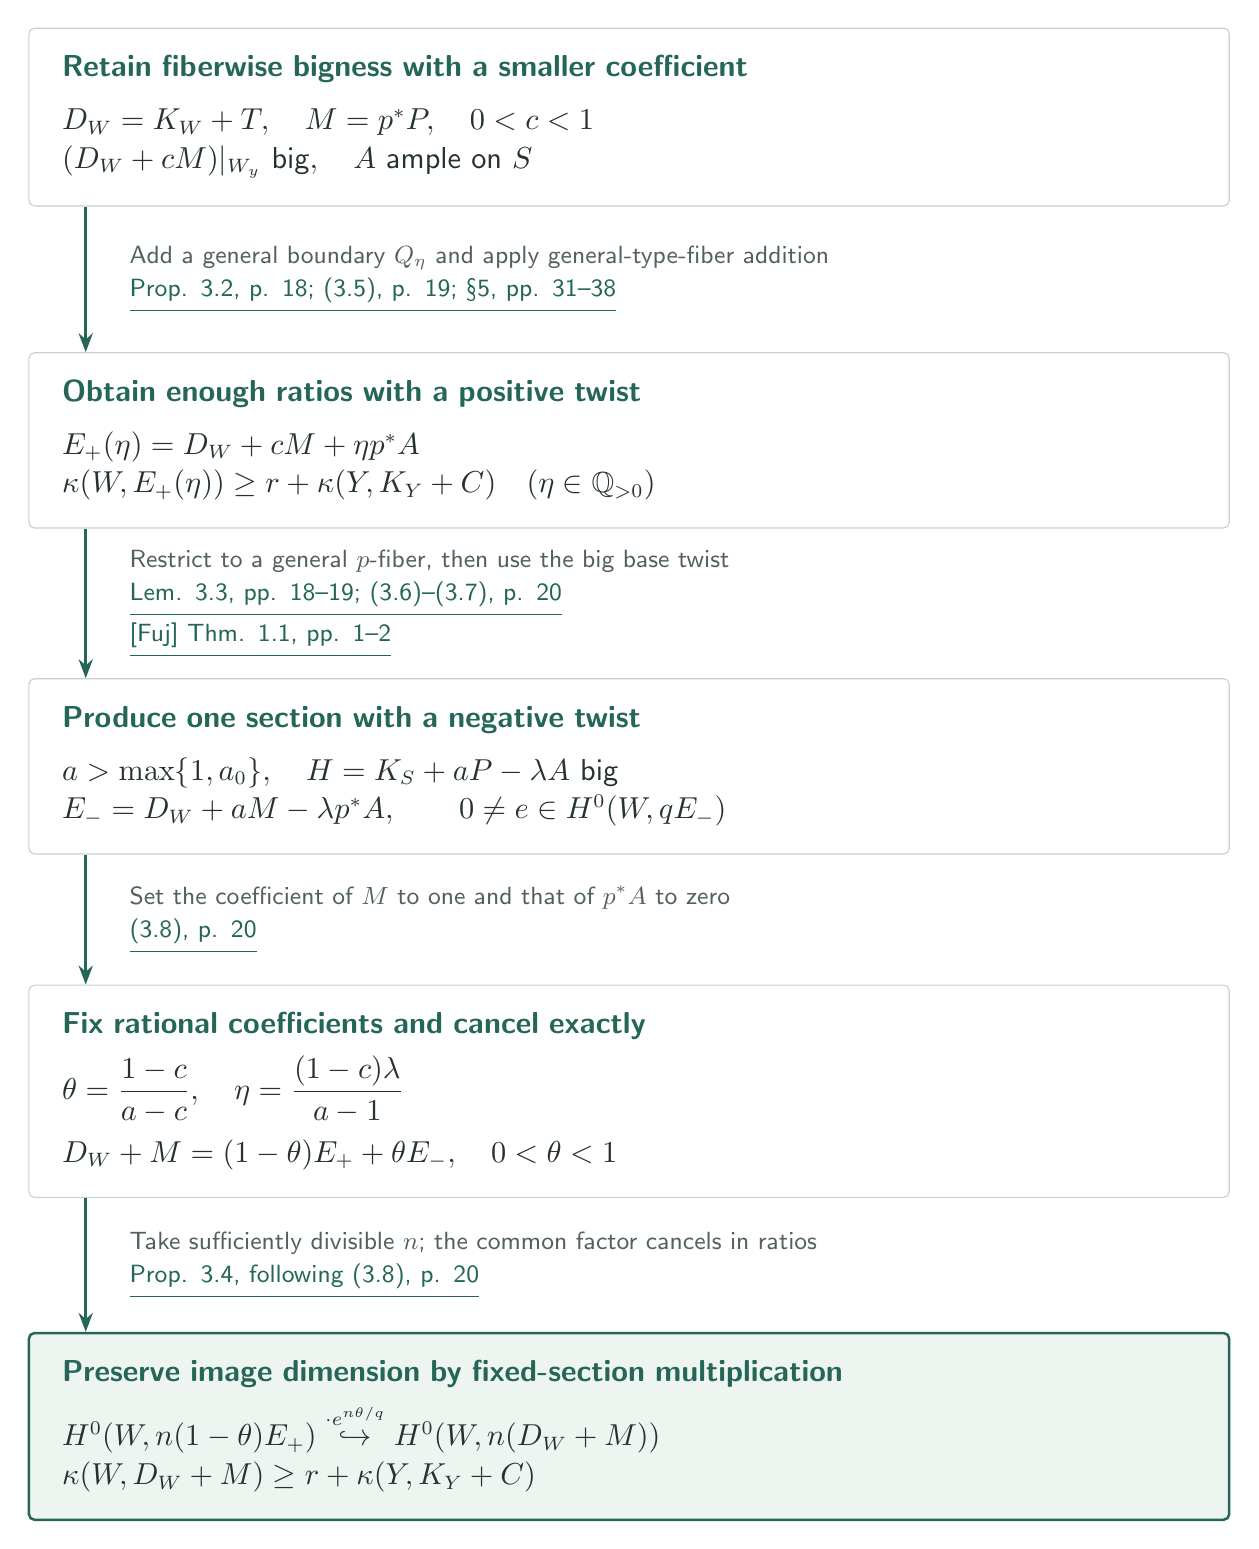
\begin{tikzpicture}
\node[card] (a) {\heading{ファイバー上のbignessを少し残す}{Retain fiberwise bigness with a smaller coefficient}
 $D_W=K_W+T,\quad M=p^*P,\quad 0<c<1$\\
 $(D_W+cM)|_{W_y}\ \text{big},\quad A\ \text{ample on }S$};
\node[card,below=1.85cm of a] (b) {\heading{正の捻りで十分な切断の比を得る}{Obtain enough ratios with a positive twist}
 $E_+(\eta)=D_W+cM+\eta p^*A$\\
 $\kappa(W,E_+(\eta))\ge r+\kappa(Y,K_Y+C)\quad(\eta\in\mathbb Q_{>0})$};
\flow{a}{b}{\Tx{一般の境界 $Q_\eta$ を加えて一般型ファイバーの加法性を適用}{Add a general boundary $Q_\eta$ and apply general-type-fiber addition}\\\OI{Prop. 3.2, p. 18; (3.5), p. 19; \S5, pp. 31--38}}
\node[card,below=1.9cm of b] (c) {\heading{負の捻りの切断を一つ作る}{Produce one section with a negative twist}
 $a>\max\{1,a_0\},\quad H=K_S+aP-\lambda A\ \text{big}$\\
 $E_-=D_W+aM-\lambda p^*A,\qquad 0\ne e\in H^0(W,qE_-)$};
\flow{b}{c}{\Tx{$p$の一般ファイバーで非消滅を得て、bigな底の捻りを使う}{Restrict to a general $p$-fiber, then use the big base twist}\\\OI{Lem. 3.3, pp. 18--19; (3.6)--(3.7), p. 20}\\\Fuj{[Fuj] Thm. 1.1, pp. 1--2}}
\node[card,below=1.65cm of c] (d) {\heading{有理係数を固定して正確に相殺する}{Fix rational coefficients and cancel exactly}
 $\displaystyle\theta=\frac{1-c}{a-c},\quad\eta=\frac{(1-c)\lambda}{a-1}$\\[5pt]
 $D_W+M=(1-\theta)E_++\theta E_-,\quad0<\theta<1$};
\flow{c}{d}{\Tx{$M$の係数を1にし、$p^*A$の係数を0にする}{Set the coefficient of $M$ to one and that of $p^*A$ to zero}\\\OI{(3.8), p. 20}}
\node[result,below=1.7cm of d] (e) {\heading{固定切断の乗法で像の次元を保持}{Preserve image dimension by fixed-section multiplication}
 $H^0(W,n(1-\theta)E_+)\overset{\cdot e^{n\theta/q}}{\hookrightarrow}H^0(W,n(D_W+M))$\\
 $\kappa(W,D_W+M)\ge r+\kappa(Y,K_Y+C)$};
\flow{d}{e}{\Tx{十分可除な$n$を取り、共通因子を切断の比から消す}{Take sufficiently divisible $n$; the common factor cancels in ratios}\\\OI{Prop. 3.4, following (3.8), p. 20}}
\end{tikzpicture}

\end{document}
